Due to bitcoin's use in the black market for illicit activities, several attempts have have been undertaken both by law enforcement agencies and computer science researchers to de-anonymize the network. In this context, the aim is not to de-anonymize all Bitcoin users, but rather to identify common patterns of use. By using a passive analysis of a publicly available dataset, the limits of anonymity when using Bitcoin are demonstrated. Let’s look at the latest developments towards this end.

\section{By Law Enforcement Agencies}
The first legal issue occurred in May 2013 when bitcoins belonging to Mt.Gox were seized by the federal authorities in the US for violating money transfer regulations \cite{seize}. Then in October 2013, Silk Road a drug market website was taken down by the FBI \cite{silk}. Silk Road was a notorious website that dealt in drugs, fake IDs, ordered hits etc. Soon after this incident, Silk Road 2.0 became available backed by the former administrators of Silk Road. It too was shut down by the authorities. In February 2014, 744,000 bitcoins were stolen from Mt.Gox one of the largest bitcoin exchanges. The thief's identity still remains unknown. 

\section{Research on the Bitcoin Network}

\subsection{Using Multi-input transactions}
Multi-input transactions can be used to trace bitcoin activity back to a user.  This approach was adopted by Androulaki, Elli, et al. Multi \cite{anony}. A Multi-Input transaction is one where multiple bitcoins have to be spent in order to procure a product.

\begin{center}
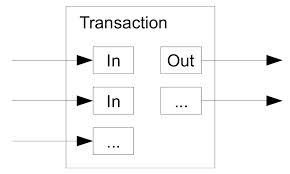
\includegraphics[scale=0.5]{images/multi.jpeg}
\end{center}

\begin{enumerate}
\item User u has 2 BTC that have value 10B(BTC1) and 20B(BTC2)
\item He wants to buy something for 25B from BTC(Dest)
\item Bitcoin clients choose a set of BTCs from u’s wallet and perform a multi-input transaction. ie. transaction from multiple BTCs. 
\item So, if we look at the block chain and observe a multi input transaction from multiple BTCs, they are from same user. (Different users cannot participate in a single transaction). So now we know that BTC1 and BTC2 are the same user.
\end{enumerate}

Using this approach, they were able to cluster 1,632,648 unique addresses into 1,069,699 addresses. To obtain further refinement, the researchers used the concept of “change” from bitcoin transactions which is as follows:

\begin{enumerate}
\item To collect the change 5B, a "shadow" address is created for u. This BTC(Shadow) is created internally by bitcoin and is never reused.
\item So, we examine the output to a transaction. If one of the address is something that has never occurred in the chain before, we know it is a shadow address. 
\item Therefore the transaction will be form 
BTC1+BTC2 -> BTC(Shadow) ,BTC(Dest)
\end{enumerate}

So, now we know that BTC1, BTC2 and BTC(Shadow) are the same user. Using this second heuristic, they were able to further cluster the 1,069,699 address into 693,051 addresses. This represents grouping approximately 58\% of bitcoin addresses with an average of 11.5 address per user.

\subsection{Using voluntarily disclosed information}
In another paper, researches made use of voluntarily disclosed information to track down users \cite{volun}.

\subsubsection{Bitcoin Faucet}
Bitcoin Faucet is a website where users can donate Bitcoins that will be redistributed to other users after breaking them into smaller pieces. To prevent fraud, Bitcoin Faucet publishes a list of recent donations along with the IP addresses of the donors. Researchers mined this list and used it in their network analysis. The public keys that were generated from here were searched in the block chain. From there, the researchers were able to put together a map of geolocated IP addresses belonging to users who receive bitcoins over a period of one week. They also put together a map of users who are linked by a path (a path between two nodes exists if a transaction has occurred between the two nodes). The path does not include the transaction to the Bitcoin Faucet. 

\begin{center}
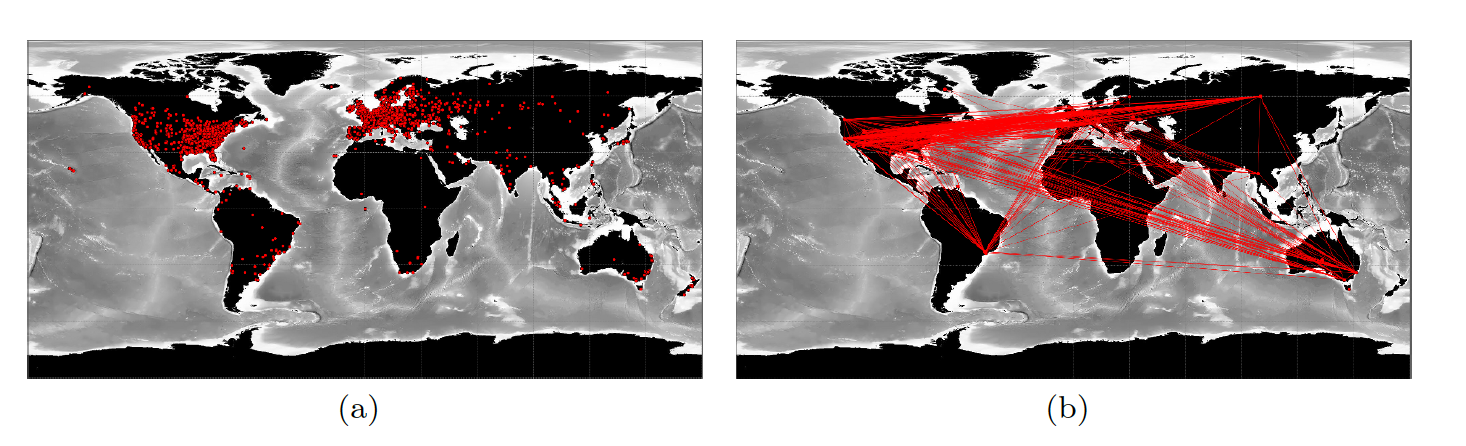
\includegraphics[scale=0.5]{images/map.png}
\end{center}

\subsubsection{Bitcoin Forums}
Many users post their experiences on numerous bitcoin forums. Sometimes, they also reveal their public key along with their comments. Public keys in Bitcoin start with the digit one and are thirty three characters in length. These can be indexed by a search engine. The researchers collected all such publicly listed public keys. They were also able to scrape public keys of users from twitter. By observing the usage of these public keys in the block chain and then obtaining the user details from the public forums, de-anonymization of users is possible.

\subsubsection{Egocentric Analysis and Visualization}
WikiLeaks publicly announced that they were accepting anonymous donations via bitcoins. They also published their public key for the users to be able to send donations. The researchers used network visualization and analysis tools to investigate the flow of bitcoins to and from WikiLeaks's public key. They were able to put together this graph representing a sub-network of all users who had contributed to WikiLeaks:

\begin{center}
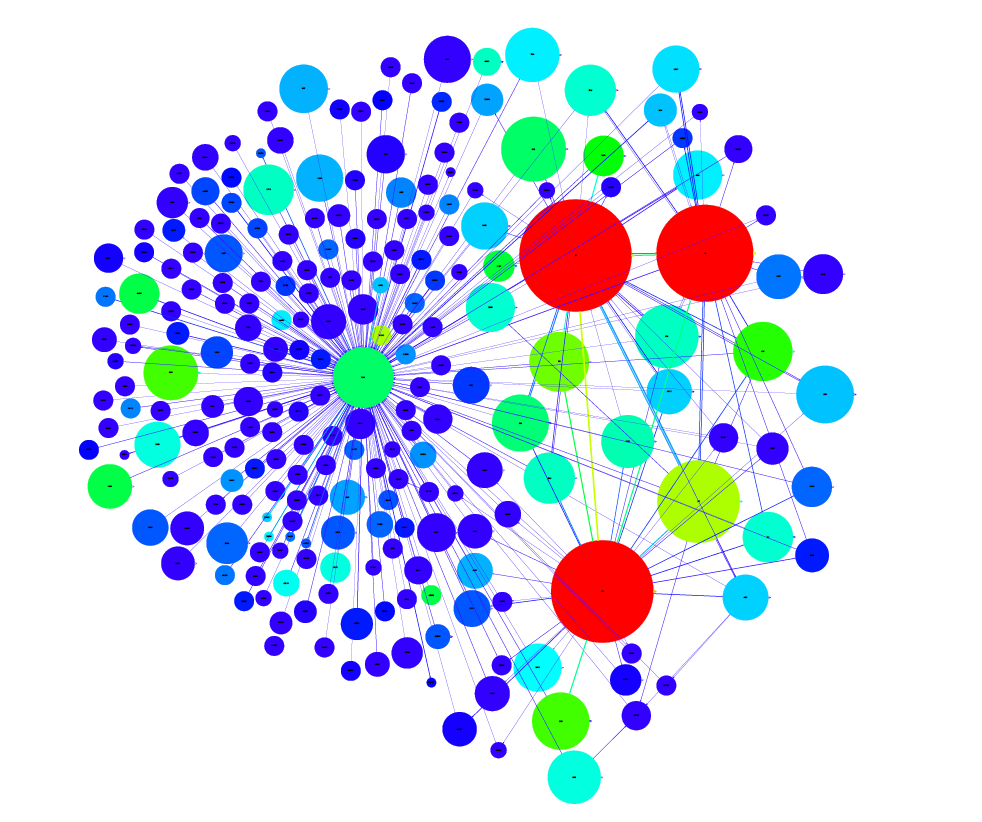
\includegraphics[scale=0.5]{images/wiki.png}
\end{center}

\subsubsection{Determining Users using addresses of Bitcoin Exchanges}
If we have identified a Bitcoin Exchange by obtaining their private keys, we can obtain a list of almost all users who have exchanged money and bought bitcoins through that exchange. The exchange is the point of origin of the bitcoin. A new public key never seen before in the block chain originates at this point. Starting from the exchange, the users found the shortest path to a user where the bitcoin went. By combining other publicly disclosed information, they were able to trace the flow of the bitcoin and pinpoint it to a user. Bitcoin exchanges collect a user’s real name and email address before exchanging real money for bitcoins. So,if a law enforcement agency subpoenas the exchange, the user’s identity along with his complete transaction history will be available to the authorities.